% !TEX root = ../../../alg_num_theory.tex
% 9 - 28 - 2009
\newpage
\subsection{Fractional Ideals, Dedekind Rings, Ideal Class Groups\label{sec:620_6}}

Let $A$ be a Dedekind domain (that is, $A$ is a noetherian integral domain integrally closed in $F=\Frac(A)$ with all nonzero prime ideals maximal and at least one nonzero prime ideal). Recall also that $J$ is a fractional ideal of $A$ if $J=x^{-1}I \subseteq H$ for some $0 \neq x \in F$ and some $A$-ideal $I$. We define $J_1 \cdot J_2$ to be the $A$-module generated by all products of elements of $J_1$ with elements of $J_2$. 

\begin{dfn}[Class Group]
If $A$ is a Dedekind ring, then $\Cl(A):=\I_F(A)/\Prin(A)$ is the class group of $A$.
\end{dfn}

Our goal is to prove the following theorem:

\begin{thm}
The set $\I_F(A)$ of all fractional ideals of $A$ forms a multiplicative group with subgroup $\Prin(A)=\{Ax \colon 0 \neq x \in F\}$. Moreover, every fractional ideal of $A$ can be written uniquely as a product of prime ideals.
\end{thm}

\pf \\

\noindent \emph{Step 1:} Every maximal ideal $\m$ of $A$ is invertible. [That is, nonzero prime ideals are invertible.] 
	\[
	\m' := \{ x \in F=\Frac(A) \colon x\m \subseteq A\}
	\]
	
\noindent Now certainly $A \subseteq \m$. Now if $0 \neq \beta \in \m$, then $\m' \subseteq \frac{1}{\beta} A$. But $\frac{1}{\beta}A$ is a nonzero noetherian $A$-submodule of $F$ (it is isomorphic to $A$ itself). Therefore, $\m'$ is a nonzero noetherian $A$-submodule of $F$ and is then a fractional ideal. We want to show that $\m\m'=A$. We know $\m \subseteq \m\m' \subseteq A$. But $\m$ is a maximal ideal of $A$ so there are only two possibilities: $\m\m'=A$ or $\m\m'=\m$. Suppose $\m\m'=\m$. Choose $x \in \m'$. Now $x\m \subseteq \m\m'=\m$. But then $x^2\m \subseteq x\m \subseteq \m$ and so $x^d \m \subseteq \m$. So if $0 \neq d \in \m$, $x^nd=p_n \in \m$ for some $p_n \in \m$. This shows that the ring $A[x]$ is generated by $A$ and $x$ and is contained in $\frac{1}{d}A$. But $\frac{1}{d}A$ is a finitely generated $A$-module. This forces $A[x]$ is a finitely generated $A$-module so that $x$ is integral over $A$. But $A$ is Dedekind so that $x \in A$. Thus, if $x\in \m'$ then $x \in A$. So $\m'=A$.


Now if $0 \neq a \in \m$, then $Aa$ contains a finite product product $P_1P_2 P_n$ of prime ideals. [Any noetherian integral domain has this property.] To see this, let $\Phi$ be the set of all nonzero ideals $I$ of $A$ which do not contain such a product. Suppose $\Phi$ is nonempty. Since $A$ is noetherian, there is an element $J$ of $\Phi$ which is maximal in the inclusion order on $\Phi$. Now $J \neq A$ as $A$ is a empty product of prime ideals. Moreover, $J$ cannot be a maximal ideal as then it would be prime and hence contain a prime ideal (itself). Then $J$ is a proper non-maximal ideal. Now clearly $J$ cannot be prime, so there exist $x,y \in A \setminus J$ with $xy \in J$. Now $J \not\subseteq (J,x)$ so by maximality, $(J,x)$ contains a product of prime ideals as $(J,x) \notin \Phi$. Similarly, $(J,y)$ contains a product of primes. Suppose $(J,x) \supseteq P_1P_2\cdots P_n$ and $(J,y) \supseteq Q_1Q_2\cdots Q_m$, all nonzero prime ideals. Then $P_1P_2 \cdots P_n Q_1 Q_2 \cdots Q_m \subseteq (J,x)(J,y)=J+Jx+Jy+Axy \subseteq J$, a contradiction. 


We were trying to show $\m\m'=\m$ is impossible. Take $0\neq a \in \m$. Certainly, $\m \supseteq Aa \supseteq P_1\cdots P_n$ for some primes $P_i$ and $n$ minimal. If $P_i \not\subseteq \m$ for all $i$, then there is a $\gamma_i \in P_i \setminus \m$. Look at $\gamma:=\gamma_1 \cdots \gamma_n$. Now $\gamma \in P_1\cdots P_n \subseteq \m$. Now $\gamma \notin \m$ as $\m$ is prime. Then $P_i \subseteq \m$ for some $i$, a contradiction. But $P_i$ is maximal as $A$ is Dedekind and then $\m=P_i$ for some $i$. Without loss of generality, $\m=P_1$. Look at $B=P_2 \cdots P_n$. We know that $Aa \not\supseteq B$ as we chose $n$ minimal. But $Aa \supseteq \m B=P_1P_2 \cdots P_n$. Choose $\beta \in B$ with $\beta \notin Aa$. Now $\m \beta\subseteq \m B = P_1\cdots P_n \subseteq Aa=aA$. Therefore, $\m \beta a^{-1} \subseteq A$. Hence, $\beta a^{-1} \in \m=\{\alpha \in F \colon \alpha \m \subseteq A\}$. Now $\beta \subseteq \m' a$ but we supposed $\m'=A$. Then $\m' a=Aa$, a contradiction since $\beta \notin Aa$. \\

\noindent \emph{Step 2:} We finish the proof that fractional ideals form a group: every fractional ideal can be written uniquely as a product of powers of distinct prime ideals, i.e. $I=P_1^{e_1} P_2^{e_2} \cdots P_n^{e_n}$. Since we can invert prime ideals (they are maximal) then we will have the desired group structure. \\

\noindent Suppose $J$ is a fractional ideal. Clearing denominators, $J$ is a finitely generated $A$-submodule of $F$. That is, $J=(dJ)(Ad)^{-1}$ for some $0 \neq d \in A$ with $dJ \subseteq A$. So to show existence of a factorization, we can reduce to the case where $J $ is an ideal of $A$. Say $\Psi$ is the set of nonzero $A$-ideals which are \emph{not} products of a finite number of prime ideals. Suppose this is nonempty. Since $A$ is noetherian, there is a maximal element in the partial order on $\Psi$ in inclusion, call this maximal element $I \in \Psi$. Now $I \neq A$, which is the empty product. Then $I$ is contained in some maximal ideal, say $\m$. Now $I\m' \subseteq \m\m'=A$, where $\m'$ is the inverse of $\m$. We know $A \subseteq \m'=\{\alpha \in F \colon \alpha \m\subseteq A\}$. Then $I=IA\subseteq I \m' \subseteq \m\m'=A$. If $I\m'$ is a product of primes, as $\m'$ is a product of primes, then by multiplication by inverses, we obtain $I$ as a product of primes. So we need only show $I \subsetneq I \m'$. Suppose $I=I\m'$. For all $x \in \m'$, using the same argument as before, we have $x^nI \subseteq I$. For any $0 \neq d \in I$, $x^nd \in I$ so that $x^n \in \frac{1}{d} I$. Now $A[x] \subseteq A + \frac{1}{d} I$ is a finitely generated $A$-module. Then $x$ is integral over $A$ so that by Dedekind-ness, $x \in A$. But then $\m' \subseteq A$, a contradiction. So $I \not\subseteq I \m'$ is not in $\Psi$. Then $I\m'$ is a product of primes and hence after multiplication by $\m$, we obtain $I$ as a product of primes, so $I \notin \Psi$, a contradiction. \\

\noindent \emph{Step 3:} We need to show uniqueness of this prime decomposition. \\

\noindent Suppose $I=P_1^{a_1}\cdots P_n^{a_n}=Q_1^{b_1} \cdots Q_m^{b_m}$, where $P_i,Q_i$ are prime and $a_i,b_j >0$. Now $P_1 \supseteq P_1^{a_1}\cdots P_n^{a_n}=Q_1^{b_1} \cdots Q_m^{b_m}$ so that $P_1 \supseteq Q_j$ for some $j$. By maximality, $P_1=Q_j$ for some $j$. Multiply by $P_1^{-1}=Q_j^{-1}$ and continue inductively. \qed \\

\begin{ex}
\begin{enumerate}[(i)] \hfill
\item We first prove a way of constructing many examples of Dedekind rings. 
\begin{thm}
Suppose we have 
	\[
	\begin{tikzcd}
	 A' \arrow[draw=none]{r}[sloped,auto=false]{\subseteq} \arrow[dash]{d} & L \arrow[dash]{d}{\text{fin. sep.}} \\
	 A  \arrow[draw=none]{r}[sloped,auto=false]{\subseteq} & F=\Frac(A)
	 \end{tikzcd}
	\]
where $A$ is Dedekind and $A'$ is the integral closure of $A$ in $L$. Then $A'$ is Dedekind.
\end{thm}

\pf Certainly $A'$ is an integral domain and is integrally closed as $\Frac(A')=L$. Now $A'$ is a finite $A$-module (since $L/F$ is finite separable) so $A'$ is a noetherian ring. It remains to show that all primes $P'$ of $A'$ are maximal and $A'$ is not a field. If $P'$ is nonzero, then $P:= P' \cap A \subseteq A$ is a prime ideal of $A$. Choose $0 \neq x \in P'$. Look at the polynomial of minimal degree with $x$ satisfies: $x^m+a_{m-1}x^{m-1} + \cdots + a_0=0$ with $a_i \in A$. Then $a_0 \neq 0$ as $a_0= -(x^m + a_{m-1}x^{m-1} + \cdots + a_1x) \in P'$ since $x \in P'$. Then $0 \neq a_0 \in P=P' \cap A$ is a nonzero prime ideal. Now $A'/P'$ is an integral domain and a finitely generated module for the field $A/P$. But then $A'/P'$ is a field so that $P'$ is a nonzero maximal ideal. [The Going-down theorem would do this quickly.] Now $A'$ is a finitely generated $A$-module. Suppose $0 \neq Q \subseteq A$ is a prime ideal. If $QA'=A'$, then $A'=Q^{-1}A$. This implies that each $x \in Q^{-1}$ is integral over $A$. But then $Q^{-1} \subseteq A$, a contradiction. Now $A'/QA'$ is nonzero finitely generated $A/Q$-module; that is, a finitely generated commutative algebra over the field $A/Q$. Then pull back a maximal ideal to get a maximal nonzero ideal $P'$ of $A'$. \qed \\

\item The most common example we will deal with follows from the above theorem: $\Z=A$, $F=\Frac(A)=\Q$, $L$ a number field, and $A'=\co_L$. 

\item Let $k$ be an algebraically closed field, e.g. $\C$. Consider $A=k[t] \subseteq F=k(t)$. Consider $y^2=h(t):=t^3+a_2t^2+a_1t+a_0$, a cubic in $k[t]$ with no multiple roots. Assume $\char k \neq 2$ and let $L=F(y)$. Now $L$ is a separable quadratic extension since we have adjoined a square root of a cubic polynomial. It turns out $A'$, the integral closure of $A$ in $L$, is $A \oplus Ay$. This is an affine ring of the elliptic curve defined by $y^2=h(t)$.


Anytime we have a diagram as above, i.e. the integral closure in a finite separable extension, if $P$ is a nonzero prime ideal of $A$, then $PA'=p_1^{e_1}\cdots p_s^{e_s}$ as fractional ideals $A'$-ideals with the $p_i$ distinct primes of $A'$. Now let $e_i=e(P_i/P)$ is the ramification degree and $f_i$ is the residue field extension degree, which is $[A'/p_i: A/P]$. Next time we shall see $\sum_{i=1}^s e_if_i= [L:F]$.


Returning to the affine ring $A'=A + Ay$, $E: y^2=h(t)$ and $A=k[t]$. We claim the prime ideals of $A'$ are of the form $p(t_0,y_0):=A(t-t_0) + A'(y-y_0)$ as $(t_0,y_0) \in k \times k$ ranges over all solutions of the equation $y^2_0=h(t_0)$. To prove this, note if $p \subseteq A'$ is a prime, $p \cap A \subseteq A=k[t]$ is a nonzero prime ideal (so it must be `linear'). But $k$ is algebraically closed so that $p \cap A$ must be of the form $k[t](t-t_0)$. What are the primes over this? Now $A'/(t-t_0)A'=k[y]/(y^2-h(t_0))$. If $h(t_0) \neq 0$, there are two distinct solutions (we are not in characteristic 2) and if $h(t_0) \neq 0$ then this is not a field and has a unique maximal ideal. Then the prime ideals of $A'/(t-t_0)A'$ give the prime ideals of $A'$: $p(t_0,y_0)$ and $p(t_0,-y_0)$ over $(t-t_0)k[t]$.

What about $\Cl(A'):=\Frac(A')/\Prin(A')$? We claim this corresponds to the group law of the elliptic curve, i.e. $\Cl(A') \cong \{\infty\} \cup E(k)$ with the usual group law (the sum of 3 points on a line is the additive identity $\infty$). The isomorphism being $p(t_0,y_0) \mapsto$ the point $(t_0,y_0)$ and $A'$ maps to $\infty$. We need to prove every fractional ideal has the same class in the class group as either $A$ or a unique prime ideal $p(t_0,y_0)$. 
        \begin{figure}[!ht]
        \centering
        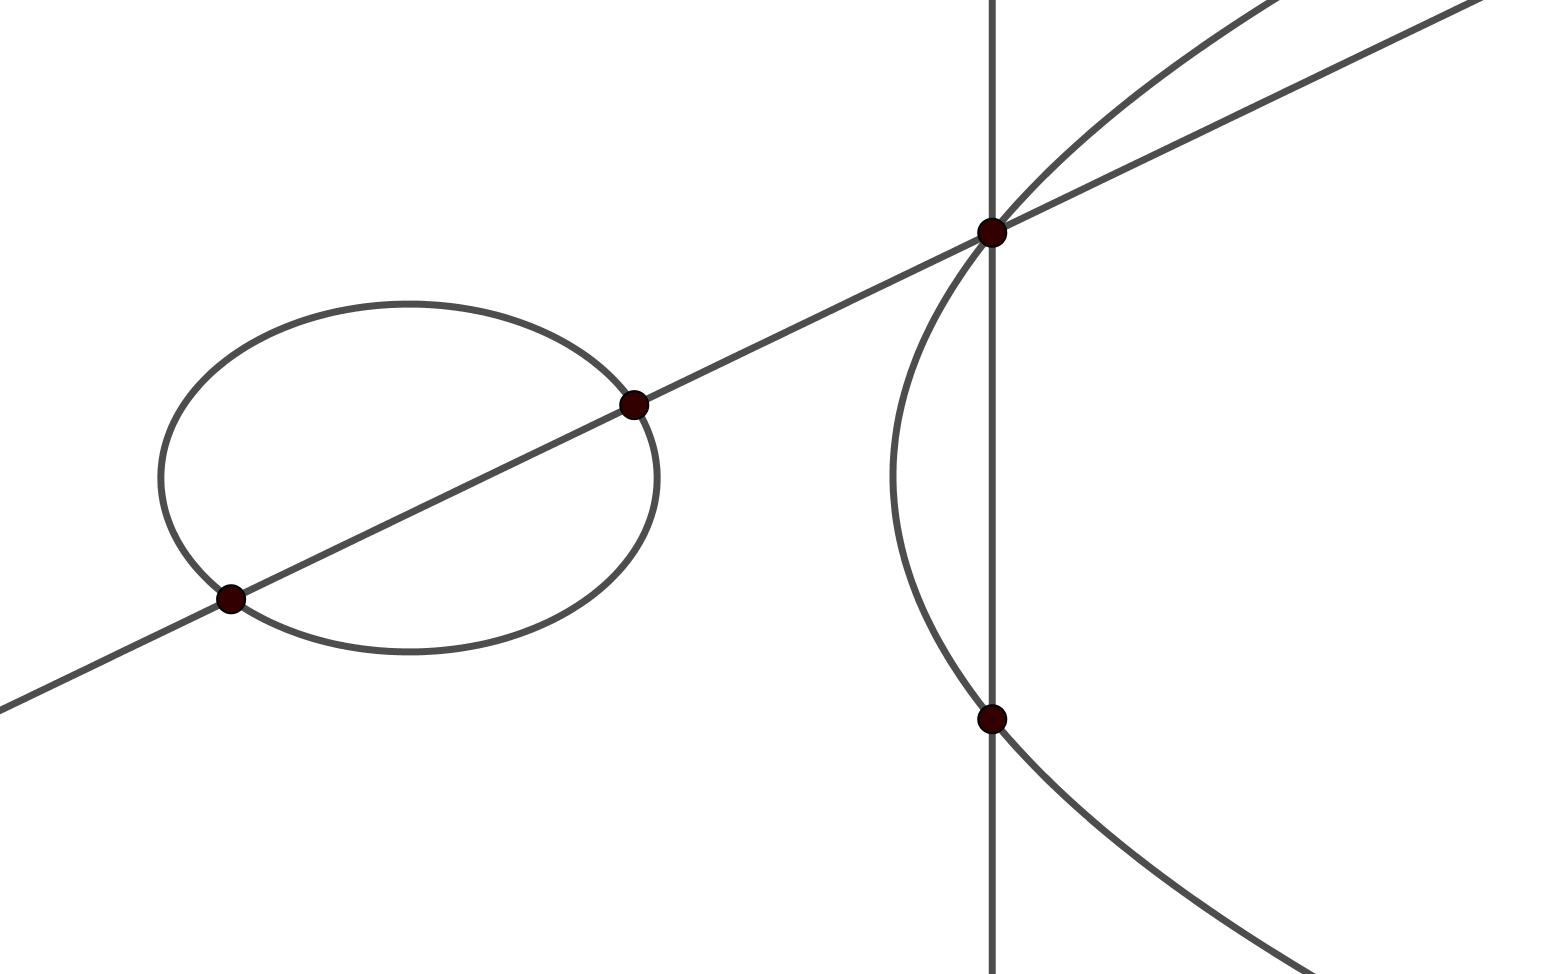
\includegraphics[width=0.5\textwidth]{images/math620/ec.png} 
        \end{figure}

The idea is this: suppose you start with two primes that correspond to two points on the elliptic curve (say the two on the `ellipse'), you want to say that the product of those two primes is linearly equivalent (adjusted by a principal ideal) to a singleton. Take the two primes and look at the equation of the line. This gives a function and look at the ideal generated by that function, its the product of the primes lying along the time (the three points). Then you have one function that generates a principal ideal whose product is the product of those three primes. Then the product of the first two primes (on the `ellipse') is linearly equivalent to the inverse of the third point on the line (along the `curve'). Consider the vertical line through the third point (hitting the `curve' at a fourth point). The product of these two ideals is the ideal generated by the function $t-t_0$ (the vertical line). Thus, the product of those two primes is a principal ideal. Therefore, the class of the third point is the inverse of the class of the fourth point. Hence, we have duplicated the group law: the product of the ideals associated to the first two points is linearly equivalent to the inverse of the prime ideal associated to the third point which is linearly equivalent to the ideal associated to the fourth point. Therefore, the product of the first two primes is linearly equivalent to the ideal associated to the fourth point.





\end{enumerate}
\end{ex}
